\documentclass[prl,twocolumn]{revtex4-1}

\usepackage{graphicx}
\usepackage{color}
\usepackage{latexsym,amsmath}
\usepackage{listings}
\usepackage{caption}
\captionsetup[figure]{font=footnotesize}
\usepackage{hyperref}
\usepackage{pygmentex} %IF ERROR, THEN LOOK BELOW
\usepackage{minted} 
\definecolor{linkcolor}{rgb}{0,0,0.65} %hyperlink
 %hyperlink%

% https://tex.stackexchange.com/questions/146264/i-cant-get-minted-package-to-work-under-ubuntu-pygments-error

\begin{document}


\title{WASC -- Deep Neural Network}





\author{Walter Zigliotto}
\author{Andrea Nicolai}
\author{Sandeep Kumar Shekhar}
\author{Camilla Quaglia}

\date{\today}


\begin{abstract}
	
The aim of this project is to develop a two layers Deep Neural Network (DNN) algorithm able to predict which sequences of a specific dataset are the secret keys. For such purpose, using a given neural network architecture, data processing techniques were used to manage the initial dataset and some DNN parameters, such as activation function, regularization, dropout and optimizer, were changed in order to improve the results. At the end, the optimal outcomes provide the efficiency of such tool on this problem.

\end{abstract}

\maketitle


\section{Introduction}

Deep Neural Network is principally a supervised machine learning technique. DNN is a discriminative model, that is the reason why it can only be used on the data classification task. Inspired by human brain activity, DNN architecture consists essentially on basic units, called “neurons”, and on their three macro-blocks organization (Fig.1):
{
\begin{itemize}
	\item Input layer: initial raw data for the neural network.
	\item Hidden layers: intermediate layer, the black box of the system, where computation is done.
	\item Output layer: result of the classification process.
\end{itemize}
}

%%%%%%%%%%%%%%%%%%%
\begin{figure}[h]
	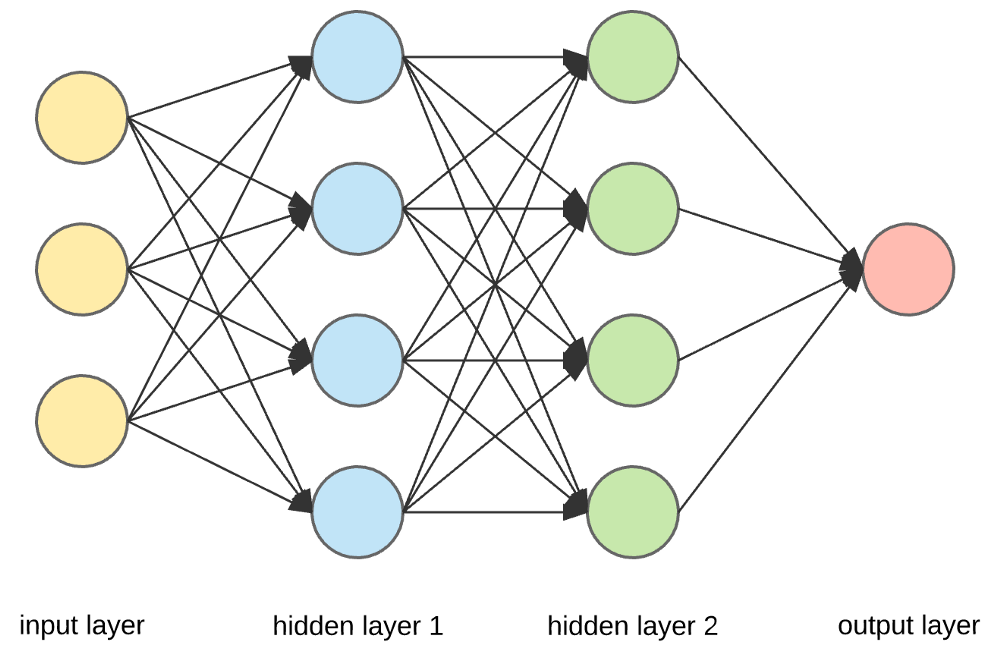
\includegraphics[width=0.33\textwidth]{DNN_structure.png}
	\caption{example of DNN structure.}
	\label{fig:y}
\end{figure}
%%%%%%%%%%%%%%%%%%%

Each neuron receives, as input, a linear combination of the previous layer neurons weighted by the edge weights, apply to the result a non-linear activation function and transmits, as output, the outcome to the next layer in turn. Formally, this process can be described by the following equation:

\begin{equation}
o_{t+1,j}(x) = \sigma \left(\sum_{r:(v_{t,r}, v_{t+1,j}) \in E}w(v_{t,r}, v_{t+1,j})o_{t,r}(x)\right)
\label{eq:simple}
\end{equation}

where \(o_{t+1,j}(x)\) is the output of the neuron, \(w(v_{t,r}, v_{t+1,j})\) is the weight of each neuron connection with \(o_{t,r}(x)\) the previous layer neuron outcome and \(sigma\) is the activation function [cit.1]. Many possible activation function (e.g., sigmoid function, Rectified Linear Unit (ReLU)) can be chosen and, along this choice depends the action potential firing of the neuron (Fig. 2):

%%%%%%%%%%%%%%%%%%%
\begin{figure}[h]
	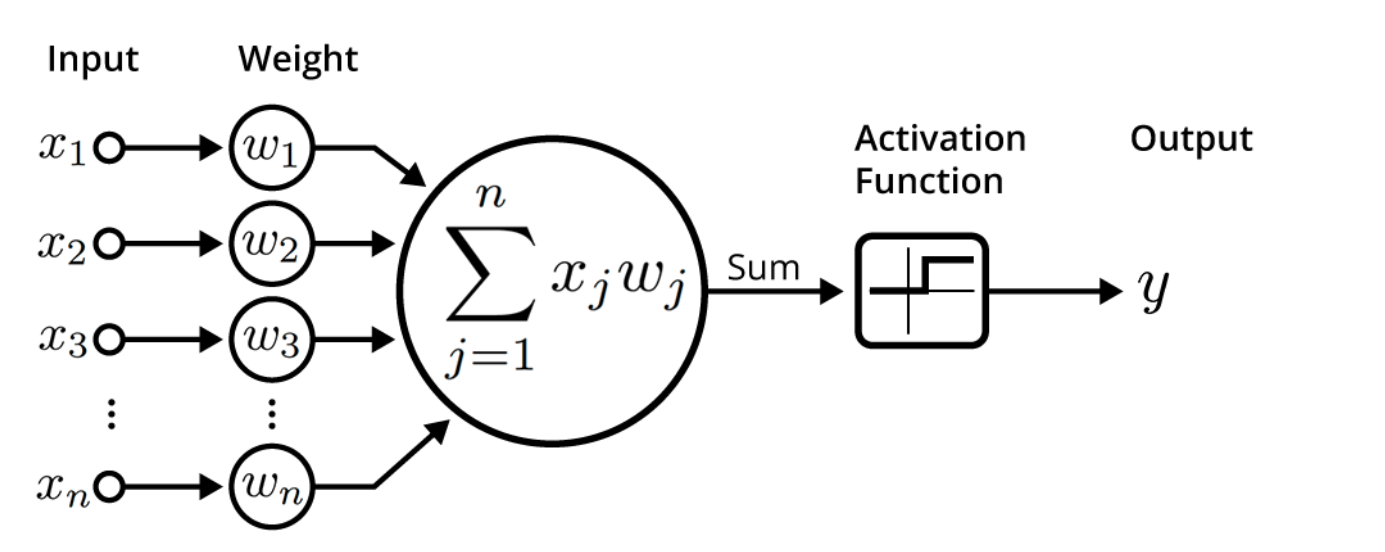
\includegraphics[width=0.44\textwidth]{Activation.png}
	\caption{example of single neuron behaviour.}
	\label{fig:y}
\end{figure}
%%%%%%%%%%%%%%%%%%%

After having define the structure, DNN has to be trained in order to improve its performance.  This procedure is done through the Stochastic Gradient Descent (SGD) method and a backpropagation algorithm. SGD is used to minimize the cost/loss function and find the optimal weights and biases. Thereafter, via backpropagation algorithm, a clever procedure that exploits the layered structure of Neural Network (NN), NN connections are rearranged to improve the results [cit. 2]. So, as to optimize the outcomes, many algorithm were attempted. \\
In order to generalize DNN to new data, avoiding overfitting problem, is also helpful to apply some regularization techniques. Primarily, Regularized Loss Minimization (RLM) methods were introduced to minimize the sum of the empirical risk and a regularization function. This regularization function acts as stabilizer of the learning algorithm, so that a tiny change of its input does not change its output much [cit. 1]. Basically, the idea is to balance the complexity of hypothesis (e.g., if the empirical risk is low, but the complexity is high, probably overfitting problem could appear). For such purpose, functions, such as L2 norm , were tried. Another method used is Dropout. The basic idea of Dropout is to prevent overfitting by reducing spurious correlations between neurons within the network by introducing a randomization. It consists of randomly “dropped out” neurons of the neural network with some probability p giving rise to a thinned network [cit. 2]. \\

(Finally, DNN is one of the promising machine learning techniques that can be applied, despite some modification, to many field, such as speech recognition and image....)





\section{Methods}
To create and train our NN we used Tensorflow 2.1.0 that already contains Keras API implemented. \textbf{REFERENCE TO TENSORFLOW DOCUMENTATION AND BELOW TO KERAS}. Moreover, we did try also a different configuration (Keras API v. 2.2.4 using Tensorflow v. 1.14.0 backend) thus leading to different results, despite the use of the same set of best parameters.\\
As previously stated our training set constitued by a sequence of 7 digits that might contain a couple of subsequences of two digits each. If so, then the correct label would be 1, thus becoming a problem of \textit{binary classification}. Each possible digit was indeed in the set $D \in  {0,1,2,3,4,5,6,7,8,9}$: therefore it fixed some constraints of the shape of the first layer. Since each number in $D$ could be present in any of the 7 position of our sequence, the \textit{input} layer needed to be composed by exactly $D \cdot L=63$ nodes. Moreover, following the instructions that were provided, we had to obey to the constraints that the \textit{first} and \textit{second} layer must be formed, at most,  respectively by $(LD/2, LD/4)$ vertices.\\
Since the problem faced is about \textit{binary classification}, the activation function in the final layer of our NN is the sigmoid one,
whose image is [0,1].
\begin{equation}
f(z) = \frac{1}{1+e^{-z}}
\end{equation}
In order to find the best set of parameters, we implemented a CV grid search, using 80\% of the whole dataset as a training set thus splitting it into 10 folds, and using a batch size of 50. Training last 40 epochs, reshuffling the set after each single iteration. Moreover for the whole research, we set the seed $1234$. Finally, after having obtained the best set of parameters, we try to predict the labels of the remaining 20\% dataset, e.g. the so-called \textit{test set}.\\
Since parameters to be tuned were only four, we thought that a good compromise would be using just only a couple of CV Grids Search: the first one would allow us to find the best \textit{Optimizer}, \textit{Regularizer (Ridge)} parameters, while the last one \textit{activation function} and \textit{Drop out} rate. All paramaters were moreover to be set equal for all the layers, except for the last before the \textit{output} one, whose nodes were burnt out according to the Drop out rate.\\
All our work consisted in applying different transformations to our dataset, and see whether it may lead to some improvements in the performance of our trained NN, always by the mean of Grid Search with Cross Validation. We expected to see that for different transformations, would correspond different set of parameters.\\
First we used the "smooth" dataset as it had been delivered to us. It was made up by 3000 entries. We expected to fall into some overfitting problems, and actually it happened as it will be shown in the results section.\\
Secondly we tried, once we had reshaped our data in a way compatible to feed the Network, to shift and rescale them. This meant that, for each of the $L*D = 63$ mentioned before, we subtracted its mean thus normalizing in order to set its standard deviation to 1. After having applied this transformation, we used Grid Search CV.\\
Lastly, we noticed that in our dataset there was an invariance of the results with respect to shift of the digits. This could be translated in the fact that if a certain sequence (e.g. $345\textbf{67}89$) contained the key, then also the $L-1$ equivalent sequences would hold it ($45\textbf{67}893$, $9345\textbf{67}8$ and so on...). In order to augment our dataset, we defined the following function that accepts in input the data and its labels:
\begin{minted}[breaklines]{python}
def expand_augment(data, label):
  S = data

  x_temp = [0] * LD  #initialize empty vectors
  y_temp = label

  p = 10**(L-1)
  j = 0
#in this way we obtain the first digit (MSD)
  while (j < L):  
    q = int(S/p)

    x_temp[j*D + (q-1)] = 1
    j += 1
    S = S - q*p
    p = int(p/10)

  x_aug  = [0] * LD * L
  x_aug  = np.reshape(x_aug, (L, LD))
  y_aug  = np.array([0]*L)
#for each combination possible by shifting
  for combination in range(L): 
  #for each possible number 
    for index in range(LD): 
      x_aug[combination][(index + combination*D)%LD] = x_temp[index]
      y_aug[combination] = label 

  return x_aug, y_aug
\end{minted}

In this way we were able to obtain a larger dataset by a factor $L-1 = 6$. As before, we trained our NN using a Cross Validation Grid Search in order to find the set of parameters that best predict the labels of the test set.

\section{Results}
\subsection{Tensorflow version:  2.1.0}
The following results are reached using the version 2.1.0 of Tensorflow.\\
The CV Grid Search, performed over the small dataset (3000 entries), finds the best parameters in the first column of table 1.\\
The model created with the best parameters above is trained over all the epochs, for both training and validation set. The accuracy reached and the loss function are shown in figure 3 and 4 respectively, where the blue line represent the training set and the orange one the validation set.
\begin{figure}[h]
	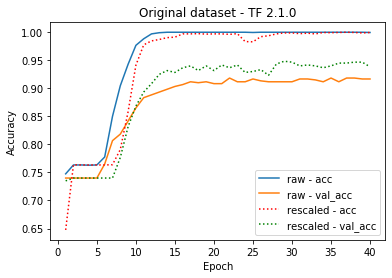
\includegraphics[width=0.40\textwidth]{small_newTF.png}
	\caption{The training set reaches the maximum for the accuracy, but there is no gain in training the network after about 10 epochs.}
	\label{fig:y}
\end{figure}
\begin{figure}[h!!!]
	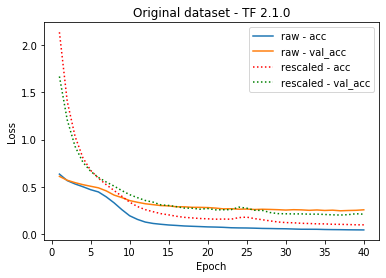
\includegraphics[width=0.40\textwidth]{small_newTFloss.png}
	\caption{}
	\label{fig:y}
\end{figure}
\\
As the green and red dashed lines in figures 3 and 4 shown, the performance of the networks improves after data rescaling, i.e. for each minibatch
\begin{equation}
x_{i} = \frac{x_{i}-E(x_{i})}{\sqrt{var(x_{i})}} 
\end{equation}
Despite there is not overfitting problems, the accuracy can be improved through 'data augmentation'. The latter procedure allows to obtain a larger dataset, with 21000 entries in our case, whose is divided in training set and validation set, like the previous one. Remember that there is invariance by shifting digits left or right, as explained in the methods section. The grid search procedure over this bigger dataset gives the best parameters in the second column of the table 1.
With the same procedure as before, two plots about the accuracy of the methods and the cost function over the epochs are obtained (figures 5 and 6 respectively). The rescaled data are always obtained though equation 3.
\begin{figure}[h]
	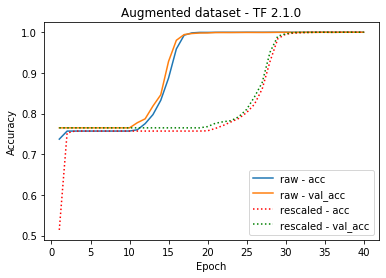
\includegraphics[width=0.40\textwidth]{aug_newTF.png}
	\caption{}
	\label{fig:y}
\end{figure}
\begin{figure}[h!!!]
	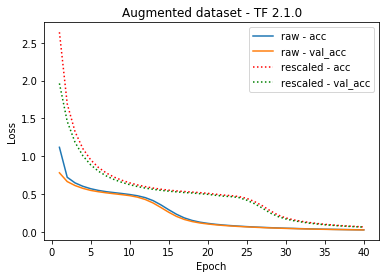
\includegraphics[width=0.40\textwidth]{aug_newTFloss.png}
	\caption{}
	\label{fig:y}
\end{figure}
\\
The plots 5 and 6 tell us that for the augmented data the network performs perfectly: the maximum accuracy (100\%) is reached, for both training and validation set.
\subsection{Tensorflow version:  1.6.0}
The same procedure described in the previous subsection, with the same set of paramenter in table 1 (even seed), produces different resuls on the same dataset, using a older version of tensorflow (1.6). \newpage
\begin{figure}[h!!!]
	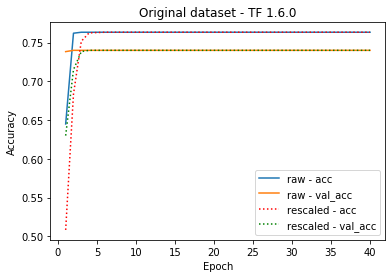
\includegraphics[width=0.40\textwidth]{small_oldTF.png}
	\caption{The accuracy remains flat for all the epochs after an initial increment, for both raw and rescaled data}
	\label{fig:y}
\end{figure}
\begin{figure}[h!!!]
	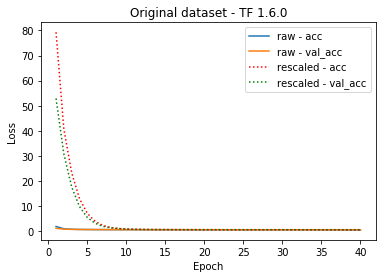
\includegraphics[width=0.40\textwidth]{small_oldTFloss.png}
	\caption{}
	\label{fig:y}
\end{figure}
In figures 9 and 10 are shown the accuracy and the loss obtained in training the augmented dataset (21000 entries) over the epochs, while figures 7 and 8 shows the results for the small dataset (3000 entries).
\begin{figure}[h!!]
	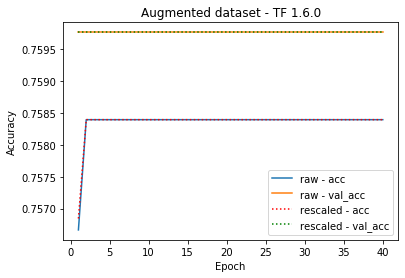
\includegraphics[width=0.40\textwidth]{aug_oldTF.png}
	\caption{The behaviour of the accuracy is the same than the one in figure 7, with an exaclty superimposing between raw and rescaled data. There is not an big improvement respect to the small dataset.}
	\label{fig:y}
\end{figure}
\begin{figure}[h!!]
	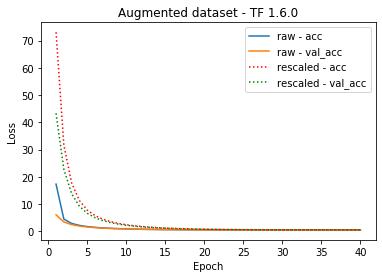
\includegraphics[width=0.40\textwidth]{aug_oldTFloss.png}
	\caption{}
	\label{fig:y}
\end{figure}
\begin{table}[ht]
\caption{Best parameters}
\begin{tabular}{c c c c}
\hline\hline
 & Small dataset & Augmented data &  \\ [0.5ex]
\hline
Optimizer & Adam & Nadam &   \\
Regularizer & 0.01 & 0.05 &  \\
Activation function & Relu & sigmoid &  \\Dropout & 0.25 & 0.15 &  \\ [1ex]
\hline
\end{tabular}
\label{table:nonlin}
\end{table}
\section{Conclusions}

PRAISE THE SUN TWICE

  





\begin{thebibliography}{99}


  
\end{thebibliography}

\end{document}





























